\section{Auswertung}
\label{sec:Auswertung}

\subsection{Nullmessung}

Wie zuvor erwähnt, muss zur Auswertung der zwei folgenden Versuchsteile der Nulleffekt berücksichtigt 
werden. Die gemessene Zeit $t_0$, sowie die Zählrate $N_0$ und die Aktivität $A_0$ sind für die beiden
Versuchsteile in Tabelle \ref{tab:null} eingetragen. Der berechnete Fehler der Zählrate ergibt sich gemäß der 
Poisson-Verteilung. Dementsprechend wird der Fehler der Aktivität mittels der Gauß'schen Fehlerfortpflanzung
bestimmt. \\
Diese Berechnung wurden mittels Python 3.6 durchgeführt. Außerdem werden die zusätzlichen integrierten 
Funktionen von den Paketen numpy, math, matplotlip und scipy verwendet. Bei allen weiteren Berechnungen und
graphischen Darstellungen wird von diesen Gebrauch gemacht. 

\begin{table}
    \centering
    \caption{Messung der Nulleffekte.}
    \label{tab:null}
    \sisetup{table-format=2.1}
    \begin{tabular}{c c c c}
    \toprule
    $\text{Messunge}$ & $ t_0 \;/\; \si{\second} $  & $N_0$ & $A_0 \;/\; \si{\per\second}$\\
    \midrule 
        $\gamma \text{-Strahlung}$ & 900 & $\num{973+-31}$ & $\num{1.08+-0.04}$\\
        $\beta \text{-Strahlung}$  & 900 & $\num{551+-23}$ & $\num{0.61+-0.03}$\\     
    \bottomrule
    \end{tabular}
\end{table}

\subsection{Absorptionskoeffizient der \texorpdfstring{$\gamma$}{}-Strahlung}

In diesem Versuchsteil wird der Absorptionskoeffizienten bei der verwendeten $\gamma$-Strahlung für die 
Stoffe Eisen Fe und Blei Pb ermittelt. In Tabelle \ref{tab:atab2} sind die Messwerte zur Bestimmung 
des Absorptionskoeffizient von Blei aufgeführt.  

\FloatBarrier
\begin{table}[h]
    \centering
    \caption{Messwerte zur Bestimmung des Absorptionskoeffizienten $\mu_\text{Pb}$ und der Größe $N\left(0\right)$ von Blei.}
    \label{tab:atab2}
    \begin{tabular}{S[table-format=1.3] S[table-format=3.0] S[table-format=4.0] @{${}\pm{}$} S[table-format=2.2] S[table-format=2.2] @{${}\pm{}$} S[table-format=1.2]}
        \toprule
        {$d / \, \si{\meter}$} & {$t / \, \si{\second}$} & \multicolumn{2}{c}{$N$} & \multicolumn{2}{c}{$\; \; \frac{N}{t} \, / \, \frac{1}{\si{\second}}$} \\
        \midrule
        0.005 & 60  & 5016 & 70.82 & 82.52 & 1.18 \\
        0.010 & 120 & 5760 & 75.90 & 46.92 & 0.63 \\
        0.015 & 180 & 4680 & 68.41 & 24.92 & 0.38 \\
        0.020 & 240 & 3907 & 62.51 & 15.20 & 0.26 \\
        0.025 & 300 & 3121 & 55.87 & 9.32  & 0.19 \\
        0.030 & 360 & 2415 & 49.14 & 5.63  & 0.14 \\
        0.035 & 420 & 1730 & 41.59 & 3.04  & 0.10 \\
        0.040 & 480 & 1428 & 37.79 & 1.89  & 0.09 \\
        0.045 & 540 & 1270 & 35.64 & 1.27  & 0.07 \\
        0.050 & 600 & 971  & 31.16 & 0.54  & 0.06 \\
        \bottomrule
    \end{tabular}
\end{table}
\FloatBarrier
\noindent

Diese Messwerte der Zählrate pro Zeiteinheit $\frac{N}{t}$ sind in Abbildung \ref{fig:afig1} halblogarithmisch gegen 
die Dicke $d$ des Absorbermaterials ausgetragen. Die Korrektur die sich aus der Nullmessung ergibt, ist als Fehlerbalken
an den einzelnen Messwerten dargestellt. Mit einer linearen Ausgleichsrechnung ergeben sich die Parameter

\begin{align*}
    a &= \num{-107,6(23)} \, \frac{1}{\si{\meter}} \\
    b &= \num{4,912(72)}      \, \frac{1}{\si{\second}} \,
\end{align*}

wobei $a$ den Absorptionskoeffizienten von Blei $\mu_\text{Pb}$ und $b$ die Größe $N\left(0\right)$ als Anzahl der eintreffenden
Teilchen pro Zeiteinheit ohne Absorber darstellt. 

\FloatBarrier
\begin{figure}[h]
    \centering
    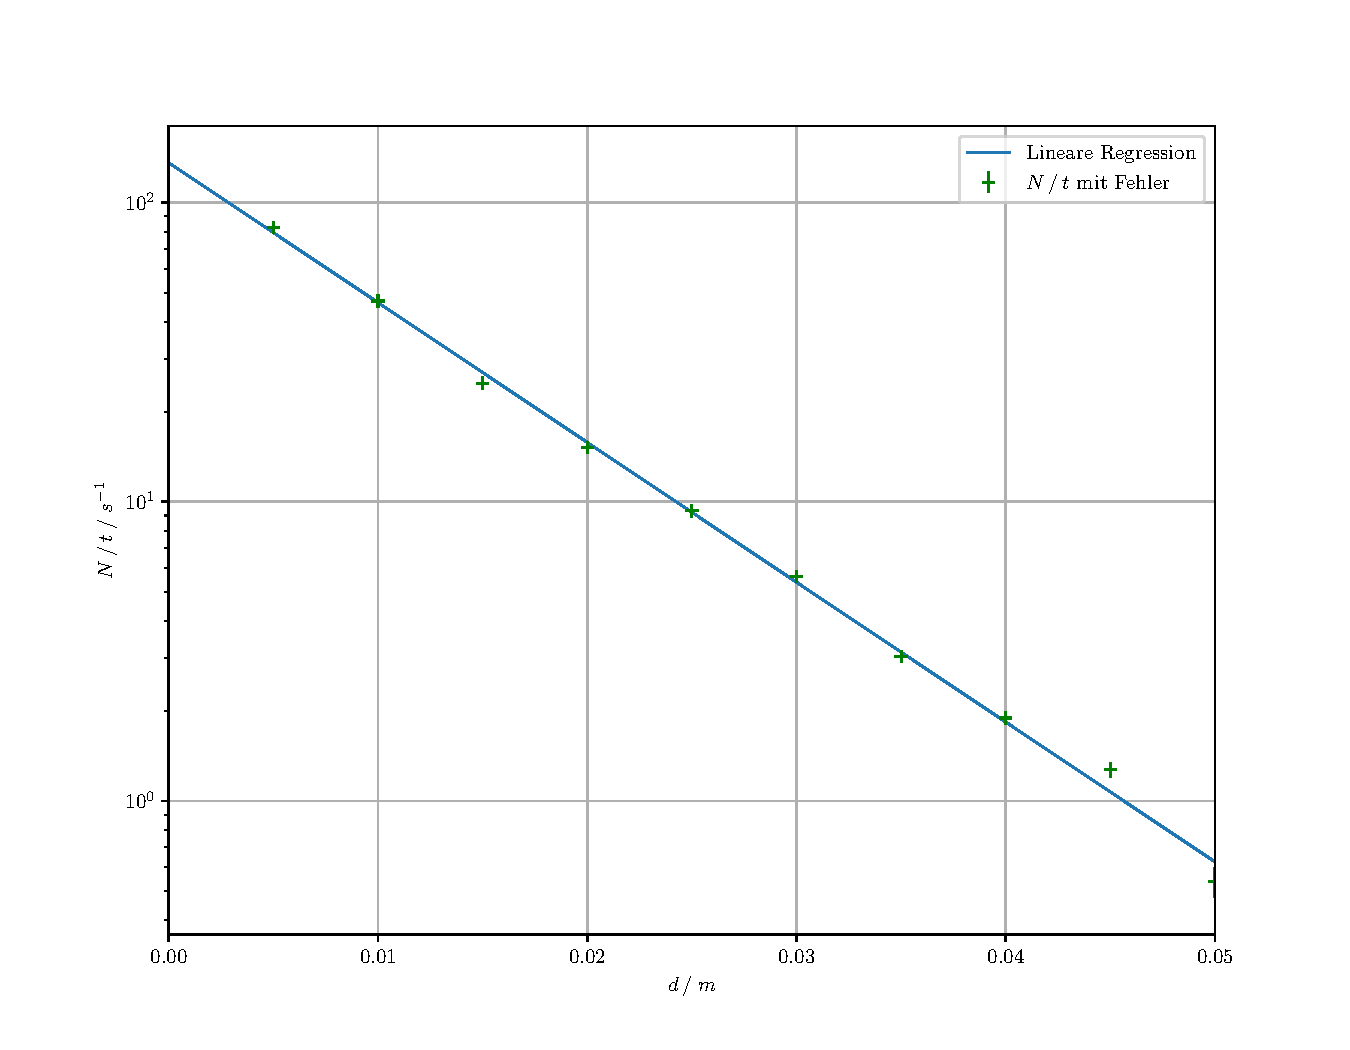
\includegraphics[width=13.5cm]{content/blei.pdf}
    \caption{Lineare Ausgleichsrechung zur Bestimmung des Absorptionskoeffizienten $\mu_\text{Pb}$ und der Größe $N\left(0\right)$ von Blei. 
    Dargestellt ist die Zählrate $N$ pro Zeiteinheit $t$ in Abhängigkeit von der Dicke $d$.}
    \label{fig:afig1}
\end{figure}
\FloatBarrier
\noindent

Die Bestimmung des Absorptionskoeffizienten von Eisen $\mu_\text{Fe}$ erfolgt analog. Die Messwerte dieser Messung sind
in Tabelle \ref{tab:atab3} dargestellt.

\FloatBarrier
\begin{table}[h]
    \centering
    \caption{Messwerte zur Bestimmung des Absorptionskoeffizienten $\mu_\text{Fe}$ und der Größe $N\left(0\right)$ von Eisen.}
    \label{tab:atab3}
    \begin{tabular}{S[table-format=1.3] S[table-format=3.0] S[table-format=4.0] @{${}\pm{}$} S[table-format=2.2] S[table-format=3.2] @{${}\pm{}$} S[table-format=1.2]}
        \toprule
        {$d / \, \si{\meter}$} & {$t / \, \si{\second}$} & \multicolumn{2}{c}{$N$} & \multicolumn{2}{c}{$\; \; \frac{N}{t} \, / \, \frac{1}{\si{\second}}$} \\
        \midrule
        0.005 & 60  & 6853 & 82.78 & 113.14 & 1.38 \\
        0.010 & 90  & 8167 & 90.37 & 89.66  & 1.00 \\
        0.015 & 120 & 8208 & 90.60 & 67.32  & 0.76 \\
        0.020 & 150 & 8078 & 89.88 & 52.77  & 0.60 \\
        0.025 & 170 & 8142 & 90.23 & 46.81  & 0.53 \\
        0.030 & 190 & 6997 & 83.65 & 35.75  & 0.44 \\
        0.035 & 210 & 6030 & 77.65 & 27.63  & 0.37 \\
        0.040 & 240 & 5674 & 75.33 & 22.56  & 0.32 \\
        0.045 & 270 & 5028 & 70.91 & 17.54  & 0.26 \\
        0.050 & 300 & 4661 & 68.27 & 14.46  & 0.23 \\
        \bottomrule
    \end{tabular}
\end{table}
\FloatBarrier
\noindent

Aus der linearen Ausgleichsrechnung in Abbildung \ref{fig:afig2} ergeben sich so die Parameter 

\begin{align*}
    a &= \num{-45,6(9)} \, \frac{1}{\si{\meter}}\\
    b &= \num{4,933(27)} \, \frac{1}{\si{\second}} \quad .
\end{align*}

\FloatBarrier
\begin{figure}[h]
    \centering
    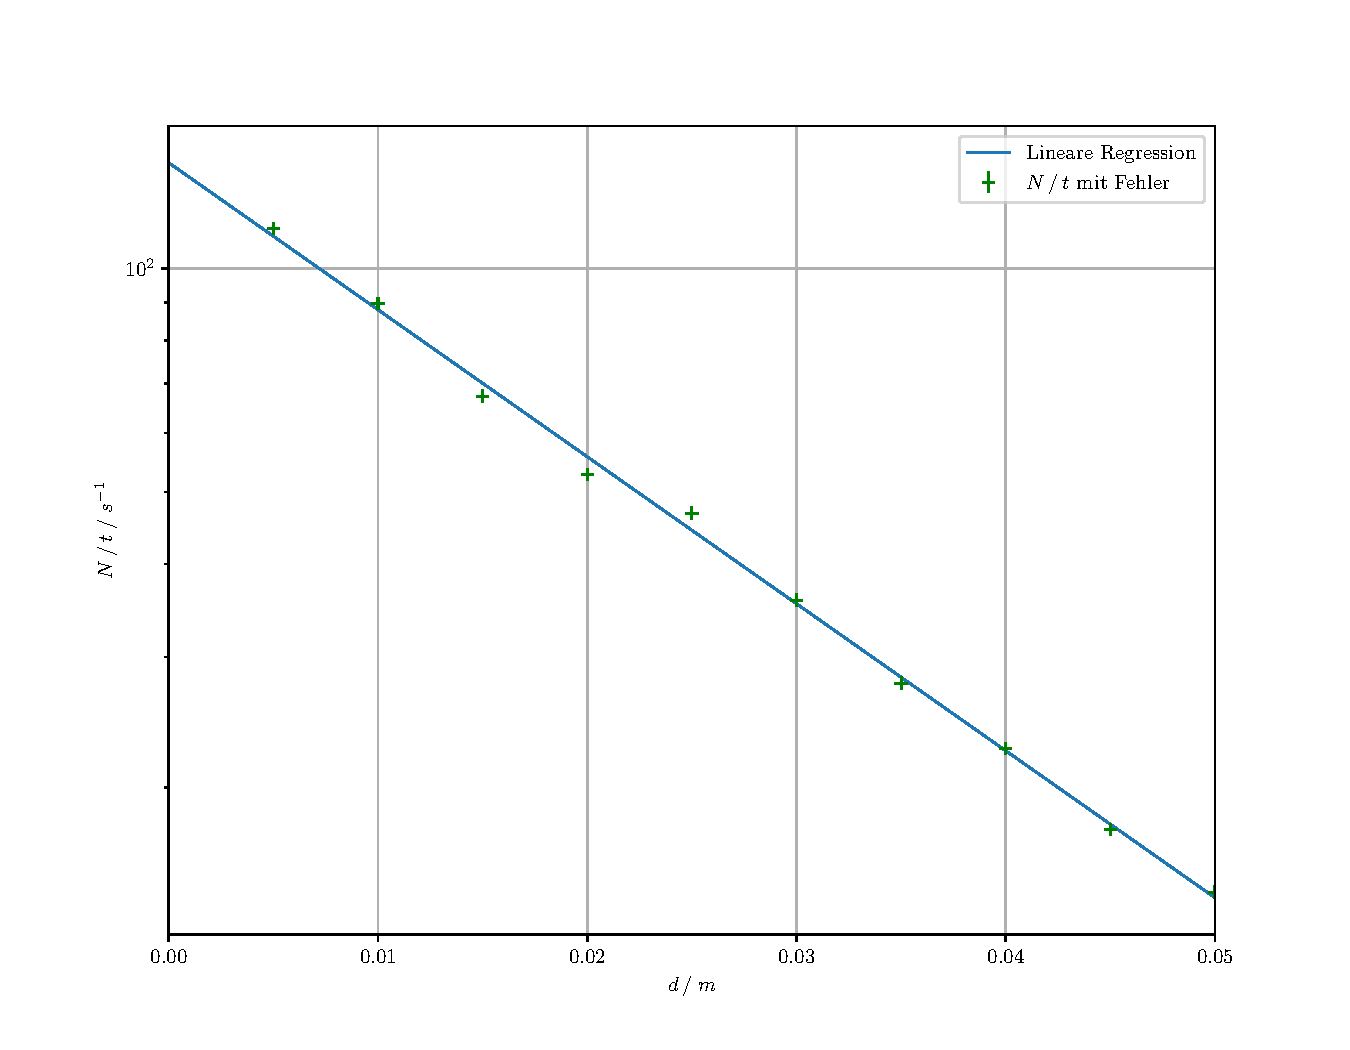
\includegraphics[width=13.5cm]{content/eisen.pdf}
    \caption{Lineare Ausgleichsrechung zur Bestimmung des Absorptionskoeffizienten $\mu_\text{Fe}$ und der Größe $N\left(0\right)$ von Eisen. 
    Dargestellt ist die Zählrate $N$ pro Zeiteinheit $t$ in Abhängigkeit von der Dicke $d$.}
    \label{fig:afig2}
\end{figure}
\FloatBarrier

\subsubsection{Berechnung des Absorptionskoeffizienten \texorpdfstring{$\mu_\text{Compton}$}{}}

Als Vergleichswert für die experimentell ermittelten Werte der Absorptionskoeffizienten von Blei und Eisen wird aus
Formel \eqref{eqn:mucompton} der Compton-Absorptionskoeffizient $\mu_\text{Compton}$ bestimmt. Dazu muss der Wirkungsquerschnitt
der Compton-Streuung $\sigma_\text{Compton}$ für $\ce{^{137}Cs}$ bekannt sein, der sich aus Formel \eqref{eqn:sigmacompton} und dem 
Energieverhältnis $\varepsilon = 1.295$ berechnet, sodass folgt

\begin{equation*}
    \sigma_\text{Compton} = \SI{2,566e-29}{\meter\squared} \quad .
\end{equation*}

Mit den stoffspezifischen Werten in Tabelle \ref{tab:atab4} ergibt sich so für den Absorptionskoeffizienten $\mu_\text{Compton}$

\begin{align*}
    \mu_\text{Compton, Pb} &= 69.351 \, \frac{1}{\si{\meter}} \\
    \mu_\text{Compton, Fe} &= 56.640 \, \frac{1}{\si{\meter}} \quad .
\end{align*}

\FloatBarrier
\begin{table}[h]
    \centering
    \caption{Stoffspezifische Werte zur Berechnung des Absorptionskoeffizienten $\mu_\text{Compton}$ [2] [3].}
    \label{tab:atab4}
    \begin{tabular}{l c c  S[table-format=1.4]}
        \toprule
        {} & {$Z$} & {$\rho / \, \si[per-mode=reciprocal]{\kilo\gram\per\cubic\meter}$} & {$M / \, \si[per-mode=reciprocal]{\kilo\gram\per\mol}$} \\
        \midrule
        {Blei}  & 82 & 11342 & 0.2072 \\
        {Eisen} & 26 & 7874  & 0.0558 \\
        \bottomrule
    \end{tabular}
\end{table}
\FloatBarrier

\subsection{\texorpdfstring{$\beta$}{}-Strahlung}

Ziel des Versuchsteil ist es die Maximalenergie aus der aufgenommenen $\beta$-Absorptionskurve zu 
bestimmen. Die gemessene Zählrate $N$, die gemessene Zeit $t$ und die Dicke $d$ der Aluminiumplatte 
sind in Tabelle \ref{tab:mess2} aufgetragen. 

\begin{table}
    \centering
    \caption{Gemessene Werte für die Aluminiumplatten.}
    \label{tab:mess2}
    \sisetup{table-format=2.1}
    \begin{tabular}{c c c}
    \toprule
    $ d \;/\; \si{\micro\meter} $ & $t \;/\; \si{\second}$ & $N$\\
    \midrule 
        482 & 1100 &   774\\
        444 & 1000 &   683\\
        400 &  900 &   642\\
        338 &  800 &   494\\
        302 &  700 &   505\\
        253 &  600 &   501\\
        200 &  500 &   794\\
        160 &  400 &  1704\\
        153 &  300 &  2037\\
        125 &  200 &  1439\\  
        100 &  100 &  2747\\ 
          0 &   50 & 22220\\       
    \bottomrule
    \end{tabular}
\end{table}

Im Folgenden wird für alle Berechnungen für die Zählrate $N$ der Poisson-Fehler angenommen.  
Werden die Werte aus Tabelle \ref{tab:mess2} in den Zusammenhang

\begin{equation*}
N = \frac{N}{t}-\underbrace{\frac{N_0}{t_0}}_{A_0}
\end{equation*}

eingesetzt, ergeben sich dabei die 
Werte in Tabelle \ref{tab:akti} für die Aktivität. 

\begin{table}
    \centering
    \caption{Errechnete Werte für Aktivität $A$ für das Material Aluminium.}
    \label{tab:akti}
    \sisetup{table-format=2.1}
    \begin{tabular}{c c}
    \toprule
    $ d \;/\; \si{\micro\meter} $ & $A_\text{Al} \;/\; \si{\per\second}$\\
    \midrule 
        482 & $\num{0.091+-0.036}$\\
        444 & $\num{0.071+-0.036}$\\
        400 & $\num{0.101+-0.038}$\\
        338 & $\num{0.005+-0.038}$\\
        302 & $\num{0.109+-0.041}$\\
        253 & $\num{0.223+-0.045}$\\
        200 & $\num{0.976+-0.062}$\\
        160 & $\num{3.648+-0.106}$\\
        153 & $\num{6.178+-0.152}$\\
        125 & $\num{6.583+-0.202}$\\  
        100 & $\num{26.858+-0.521}$\\ 
          0 & $\num{443.79+-2.980}$\\       
    \bottomrule
    \end{tabular}
\end{table}


Bei der Subtraktion können dabei auch negative Werte auftreten. Diese werden zum Betrag genommen, 
da der Logarithmus nicht für negative Werte definiert ist. 
In Abbildung \ref{fig:beta} werden die Aktivitäten halblogarithmisch gegen die Dicke $d$ aufgetragen. 

\begin{figure}
  \centering
  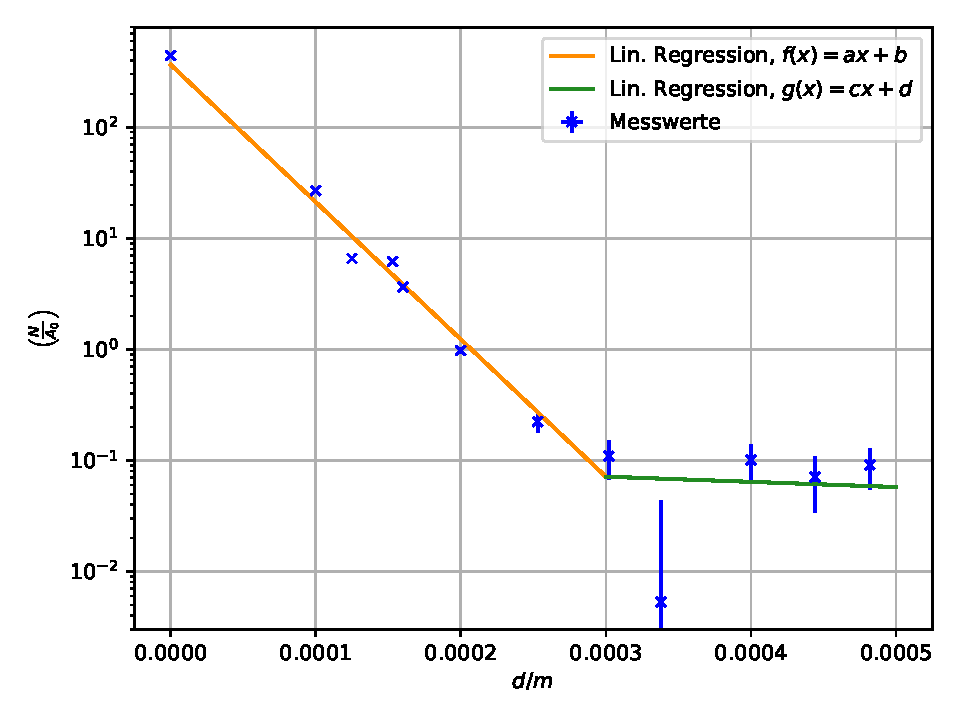
\includegraphics[scale=0.8]{content/beta.pdf}
  \caption{Lineare Regression der Messwerte zur Bestimmung von $R_\text{max}$.}
  \label{fig:beta}
\end{figure}

Um $R_\text{max}$ aus der Abbildung \ref{fig:beta} zu bestimmen werden zwei lineare Regressionen der 
Messwerte gefittet. Die eine Kurve liegt oberhalb und die andere Kurve unterhalb von $R_\text{max}$. 
Die Geradengleichungen seien dabei $f(x) = ax+b$ und $g(x) = cx+d$.

Mittels Python werden die Messwerte linear gefittet und sie ergeben sich zu 

\begin{align*}
a &= \SI{-28.48+-8.71e3}{\per\meter}, & c &= \SI{-1.08+-7.39e3}{\per\meter},\\
b &= \SI{5.91+-1.12}{\per\second}, & d &= \SI{-2.32}{\per\second}.
\end{align*}

$R_\text{max}$ wird gemäß 

\begin{equation*}
R_\text{max} = \frac{d-b}{a-c}
\end{equation*}

bestimmt, wobei dieser Wert mit der Dichte von Aluminium multipliziert werden muss. 
Damit beträgt der experimentell gemessene Werte für $R_\text{max}$:

\begin{equation*}
R_\text{max} = \SI{0.8+-0.5}{\kilogram\per\meter²}.
\end{equation*}

Die daraus resultierende Maximalenergie ergibt sich nach Formel \eqref{eqn:Emax} zu 

\begin{equation*}
E_\text{max} = \SI{0.33+-0.11}{\mega\eV}.
\end{equation*}

Zu Beachten ist die richtige Umrechnung der Massenbelegung in $\si{\gram\per\centi\meter²}$.